\documentclass[a4paper,10pt,openany]{article}
\usepackage{fancyhdr}
\usepackage[T1]{fontenc}
\usepackage[margin=1.8cm]{geometry}
\usepackage[applemac]{inputenc}
\usepackage{lmodern}
\usepackage{enumitem}
\usepackage{microtype}
\usepackage{hyperref}
\usepackage{enumitem}
\usepackage{dsfont}
\usepackage{amsmath,amssymb,amsthm}
\usepackage{mathenv}
\usepackage{amsthm}
\usepackage{graphicx}
\usepackage[all]{xy}
\usepackage{lipsum}       % for sample text
\usepackage{changepage}
\theoremstyle{plain}
\newtheorem{thm}{Theorem}[section]
\newtheorem*{thm*}{Th\'eor\`eme}
\newtheorem{prop}[thm]{Proposition}
\newtheorem{cor}[thm]{Corollary}
\newtheorem{lem}[thm]{Lemma}
\newtheorem{propr}[thm]{Propri\'et\'e}
\theoremstyle{definition}
\newtheorem{deff}[thm]{Definition}
\newtheorem{rqq}[thm]{Remark}
\newtheorem{ex}[thm]{Exercice}
\newcommand{\e}{\mathrm{e}}
\newcommand{\prodscal}[2]{\left\langle#1,#2\right\rangle}
\newcommand{\devp}[3]{\frac{\partial^{#1} #2}{\partial {#3}^{#1}}}
\newcommand{\w}{\omega}
\newcommand{\dd}{\mathrm{d}}
\newcommand{\x}{\times}
\newcommand{\ra}{\rightarrow}
\newcommand{\pa}{\partial}
\newcommand{\vol}{\operatorname{vol}}
\newcommand{\dive}{\operatorname{div}}
\newcommand{\T}{\mathbf{T}}
\newcommand{\R}{\mathbf{R}}
\newcommand{\Z}{\mathbf{Z}}
\newcommand{\N}{\mathbf{N}}
\newcommand{\C}{\mathbf{C}}
\newcommand{\F}{\mathcal{F}}
\newcommand{\Homeo}{\mathrm{Homeo}}
\newcommand{\Matn}{\mathrm{Mat}_{n \times n}}
\DeclareMathOperator{\tr}{tr}
\newcommand{\id}{\mathrm{id}}
\newcommand{\htop}{h_\mathrm{top}}


\title{\textsc{Syst\`emes dynamiques} \\ Feuille d'exercices 3}
\date{}
\author{}

\begin{document}

{\noindent \'Ecole Normale Sup\'erieure  \hfill Yann Chaubet } \\
{2021/2022 \hfill \texttt{chaubet@dma.ens.fr}}

{\let\newpage\relax\maketitle}
\maketitle

\noindent {\large \textbf{Exercice 1.} \textit{Ensemble $\omega$-limite non minimal}} \vspace{1.5mm} 

\noindent Trouver un espace m\'etrique $X$, une transformation continue $f : X \to X$ et un point $x \in X$ tels que $\omega(x)$ contienne deux parties ferm\'ees invariantes et non vides.

\vspace{0.6cm}

\noindent {\large \textbf{Exercice 2.} \textit{Croissance des orbites p\'eriodiques et entropie des applications expansives}} \vspace{1.5mm} 

\noindent Soit $(X, \dd)$ un espace m\'etrique compact et $f : X \to X$ une application continue et expansive, c'est-\`a-dire qu'il existe $\delta > 0$ tel que pour tous $x, y \in X$,
$$
\quad \sup_{n\in \N} \dd(f^n(x),f^n(y)) \leq \delta \implies x = y.
$$
Pour tout $n \in \N$, on note
$$
p_n(f) = \#\{x \in X, f^n(x) = x\}.
$$
On d\'efinit aussi le taux de croissance exponentielle de la s\'equence $p_n(f)$,
$$
p(f) = \limsup_{n \to \infty} \frac{\log(1 + p_n(f))}{n}.
$$
\begin{enumerate}
\item Montrer que $p_n(f)$ est fini pour tout $n$ et qu'on a
\begin{equation}\label{eq:lowerboundentropy}
p(f) \leq h_{\mathrm{top}}(f),
\end{equation}
o\`u $h_\mathrm{top}(f)$ est l'entropie topologique de $f$.
\item Donner un exemple d'application $f$ telle que (\ref{eq:lowerboundentropy}) soit une \'egalit\'e.
\item Montrer que pour toute matrice $A \in \mathrm{GL}(m,\mathbb{Z})$ hyperbolique (i.e. dont les valeurs propres sont toutes de module diff\'erent de $1$), on a
$$
\sum_{\substack{\lambda \in \mathrm{sp}(A) \\ |\lambda| > 1 }} \log |\lambda| \leq h_\mathrm{top}(f_A),
$$
o\`u $f_A : \T^m \to \T^m$ est l'automorphisme toral associ\'e \`a $A$.
\end{enumerate}


\vspace{0.6cm}


\noindent {\large \textbf{Exercice 3.} \textit{Codage symbolique de l'application du Chat d'Arnold}} \vspace{1.5mm} 

\noindent On consid\`ere la matrice
$$
L = \begin{pmatrix} 2 & 1 \\ 1 & 1
\end{pmatrix}.
$$
Alors $L$ induit un automorphisme $f_L : \T^2 \to \T^2$ appel\'e application du Chat d'Arnold. Alors $L$ a deux valeurs propres $\displaystyle{\lambda = \frac{3 + \sqrt{5}}{2}}$ et $\lambda^{-1}$. Les vecteurs propres associ\'es respectifs sont $\displaystyle{v = \begin{pmatrix}1 \\ 1 - \lambda^{-1}\end{pmatrix}}$ et $w = \displaystyle{ \begin{pmatrix}1 \\ -1 - \lambda\end{pmatrix}}$. On consid\`ere une partition de $\T^2$ en deux rectangles $R^{(1)}$ et $R^{(2)}$ dont les c\^ot\'es sont parall\`eles \`a $v$ ou $w$ (voir Figure \ref{fig:partition}). Alors $f_L(R^{(1)})$ se d\'ecompose en trois rectangles $\Delta_0, \Delta_1$ et $\Delta_3$ tandis que $f_L(R^{(2)})$ se d\'ecompose en deux rectangles $\Delta_2$ et $\Delta_4$ (voir Figure \ref{fig:partition}).
\begin{figure}[h!]
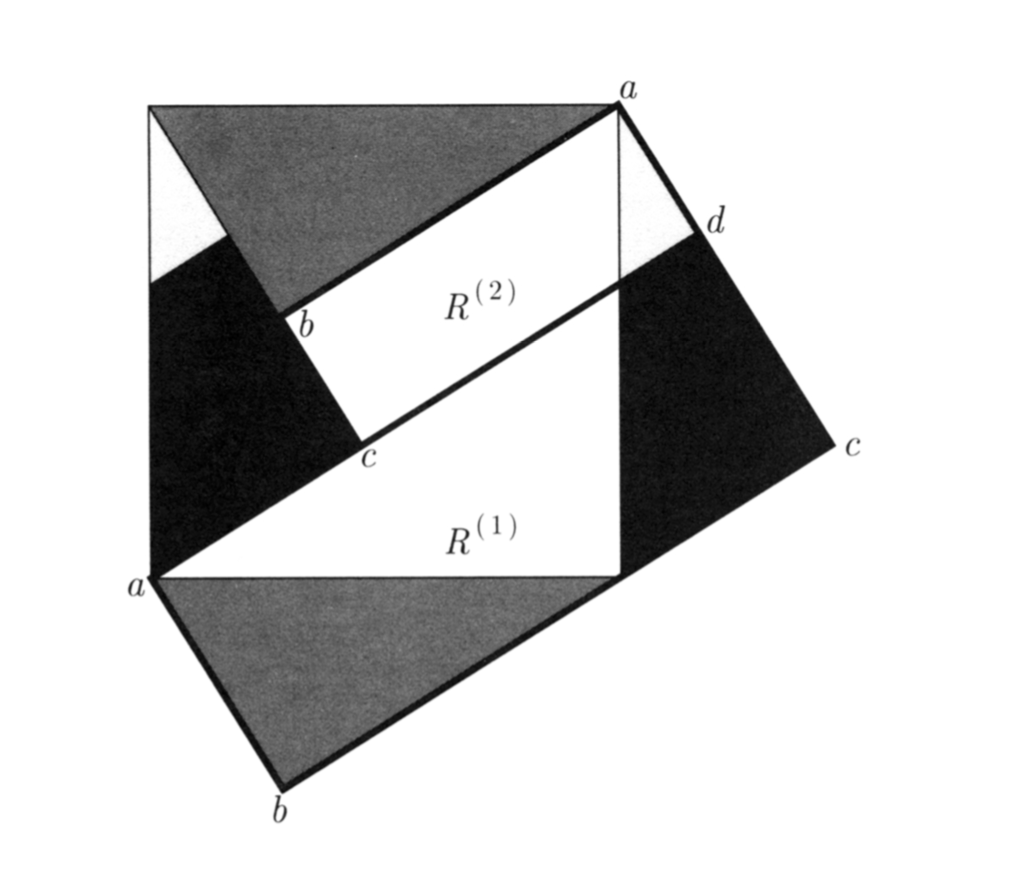
\includegraphics[width=8.95cm]{partition_torus.png}
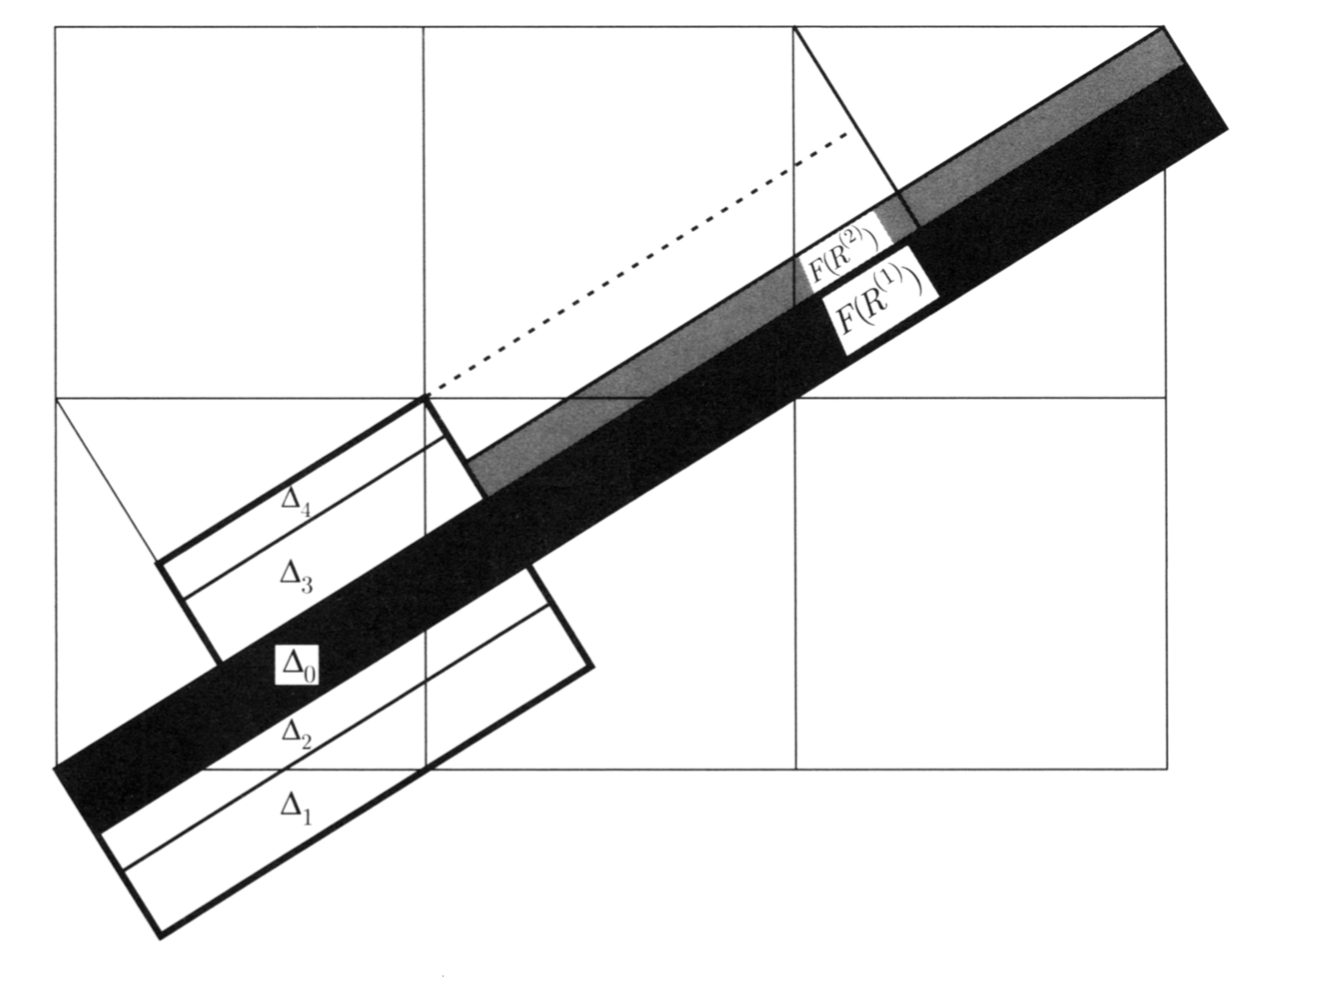
\includegraphics[width=8.95cm]{image_partition_torus.png}
\caption{Partition de $\T^2$ en deux rectangles (\`a gauche) et image des relev\'es de ceux ci par $F : x \mapsto Lx$ (\`a droite)}
\label{fig:partition}
\end{figure}
\begin{enumerate}
\item En utilisant la partition $\T^2 = \bigcup_{j=0}^4 \Delta_j$, montrer que $f_L$ est un facteur d'une cha \^ine de Markov topologique dont on pr\'ecisera la matrice de transition.
\item En d\'eduire l'entropie topologique de $f_L$.
\end{enumerate}


\vspace{0.6cm}
%%%

\noindent {\large \textbf{Exercice 4.} \textit{Fonctions z\^eta dynamiques}} \vspace{1.5mm} 

\noindent Soit $(X, \dd)$ un espace m\'etrique compact et $f : X \to X$ une transformation continue et expansive de $X$. On d\'efinit la fonction z\^eta dynamique de $f$ par
$$
\zeta_f(z) = \exp \sum_{n=1}^\infty \frac{p_n(f)}{n} z^n, \quad z \in \C, \quad |z| < \exp (- p(f)),
$$
o\`u $p_n(f)$ et $p(f)$ sont d\'efinis dans l'exercice \textbf{2}.
\begin{enumerate}
\item Montrer que $\zeta_f$ est bien d\'efinie.
\item Montrer, dans les cas suivants, que $\zeta_f$ est une fonction rationnelle admettant un p\^ole simple au point $z = \exp \left(-h_\mathrm{top}(f)\right)$, et que
$$
p_n(f) \sim \exp\left(n\htop(f)\right) \quad (n \to \infty).
$$
\begin{enumerate}
\item $X = \T$ et $f : x  \mapsto mx $ o\`u $m \in \N_{\geq 2}$.
\item $X = \T^2$ et $f = f_L$ est l'application du Chat d'Arnold.
\item $X = \Sigma_A$ o\`u $A$ est une matrice $n \times n$ \`a coefficients dans $\{0,1\}$ irr\'eductible\footnote{En particulier, par le th\'eor\`eme de Perron-Frobenius, il existe une valeur propre $\lambda > 0$ telle que $\lambda = \rho(A)$ et $\mathrm{sp}(A) \cap \{|z| \in \C,~ |z| = \lambda\} = \{\lambda, \lambda \omega, \dots, \lambda \omega^{p-1}\}$ o\`u $p \in \N$ et $\omega = \exp(2 i \pi / p)$.}, 
$$\Sigma_A = \left\{(x_j)_{j \in \Z} \in \{1, \dots, n\}^\Z ~|~ \forall j \in \Z, ~A_{x_j, x_{j+1}} = 1\right\}, $$
et $f = \sigma_A$ est le d\'ecalage sur $\Sigma_A$.
\end{enumerate}

\item Montrer que 
$$
\zeta_f(z) = \prod_{p \in \mathcal{P}} \left(1 - z^{|p|}\right)^{-1},
$$
o\`u $\mathcal{P}$ est l'ensemble des orbites p\'eriodiques de $f$, et $|p|$ d\'esigne la p\'eriode de l'orbite $p \in \mathcal{P}$.

\end{enumerate}

\vspace{0.6cm}

\noindent {\large \textbf{Exercice 5.} \textit{Toute transformation continue surjective est facteur d'un hom\'eomorphisme}} \vspace{1.5mm} 

\noindent On se donne $f : X \to X$ une transformation continue et surjective d'un espace topologique. Montrer qu'il existe un espace topologique $\widetilde{X}$, un hom\'eomorphisme $\widetilde{f} : \widetilde{X} \to \widetilde{X}$ et une surjection continue $h : \widetilde{X} \to X$ tels que $f \circ h = h \circ \widetilde{f}$.
\end{document} 
